\section{Le chiffrement symétrique}
Dans les systèmes cryptographiques utilisant des clés, il faut bien
distinguer les deux types existants : le chiffrement symétrique et le
chiffrement asymétrique. Penchons nous d'abord sur le chiffrement
symétrique. Ce type de chiffrement est aussi appelé chiffrement à clé
privée, du fait que le chiffrement se fait via une clé qui doit rester
secrète, et qui ne doit être connue que par les personnes devant
chiffrer et déchiffrer les messages. La puissance de la méthode de
chiffrement réside donc dans la difficultée de trouver cette
clé. 

Cette forme de chiffrement est la plus ancienne existante, on peut par
exemple citer le chiffre de César ou le chiffre de Vigenère. Le seul
système de chiffrement entièrement sûr et fiable, le chiffre de Vernam
est un chiffrement symétrique, où la principale difficultée, outre le
fait de devoir générer une clé de la taille du texte et complètement
aléatoire, réside dans la façon de transporter les clés.

\begin{figure}[h]
  \begin{center}
    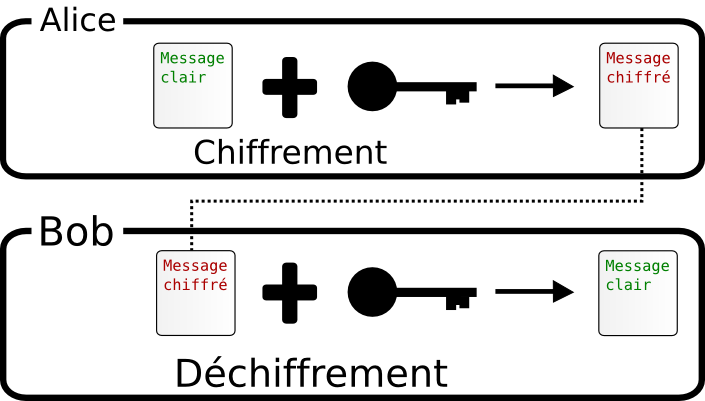
\includegraphics[scale=0.5]{images/ChiffrementSymetrique.png}
  \end{center}
  \caption{Le fonctionnement du chiffrement symétrique, les deux clés
    sont identiques.}
  \label{fig:ChiffrementSymetrique}
\end{figure}

\subsection{Le principe de Kerckhoffs\label{sec:PrincipeKerchoffs}}
Dans son article \emph{La cryptographie militaire}
\cite{CryptographieMilitaire1,CryptographieMilitaire2}, Auguste
Kerckhoffs critique le manque d'application dans l'utilisation des
techniques cryptographiques dans les armées via de nombreux exemples,
comme celui où un jour, au ministère français de la guerre, on reçut
un message à déchiffrer, mais la personne ayant connaissance de la clé
n'étant pas disponible, on demande à un officier d'essayer de
déchiffrer le message sans la clé, ce qui fut fait facilement en
quelques heures. La partie la plus connue de cet article est le
\emph{Desiderata de la cryptographie militaire}, où il énonce six
conditions pour avoir un système cryptographique fiable et utilisable
par les armées. De ces six points, le plus important est le second : «
il faut qu’il [le système cryptographique] n’exige pas le secret, et
qu’il puisse sans inconvénient tomber entre les mains de l’ennemi
». 

Ainsi, tout système cryptographique devrait avoir sa fiabilitée de la
difficultée de trouver sa clé, et non du secret de l'algorithme ; de
plus, en rendant les algorithmes publics, les cryptanalystes du monde
entier peuvent essayer de le casser ou l'améliorer. Ce principe peut
s'étendre à de sujets plus vastes que la cryptographie, comme la
sécurité en général (ce que décrit Bruce Schneier dans un article de
l'\emph{Atlantic} en 2002 \cite{HomelandInsecurity}), ainsi, la
fiabilité d'un système de sécurité ne doit pas venir du secret des
moyens mis en places (comme par exemple les logiciels utilisés, \dots
), c'est ce qu'on appelle la \emph{sécurité par l'obscurité}. Eric
Raymond étend même le principe de Kerckhoffs aux logiciels en général
lors de l'affaire Cisco (qui n'est pas en rapport avec ce travail,
pour plus d'informations, consultez le Web) en disant clairement dans
un mail\footnote{Disponible ici :
  \url{http://lwn.net/Articles/85958/}} de ne jamais faire confiance à
des logiciels à code source fermés. Cette non fiabilitée de la
sécurité par l'obscurité à déjà été prouvée par de nombreux faits : le
chiffrement des téléphones mobiles a été rendu public, de même que
l'algorithme de protection des DVD, la publication des détails de
fonctionnement des machines de votes \emph{Diebold}, \dots
\subsection{Chiffrement par bloc et par flot}
Il y a deux moyens de chiffrer les données avec les algorithmes à clé
publiques : le \emph{chiffrement par bloc} et le \emph{chiffrement
par flot} aussi appelé \emph{chiffrement par flux}. \\

\label{syst:XOR}
Tout d'abord, le chiffrement par flux traite les données commes elles
arrivent, élément par élément. Sur les systèmes informatiques et
électroniques, un élément est composé d'un bit, chaque bit est donc
traité séparément. Le chiffrement par flux le plus simple à comprendre
est sûrementle chiffrement via le \emph{ou exclusif}. Ce \emph{ou
  exclusif}, ou \emph{XOR}, est un opérateur logique définit dans
l'algèbre de Boole, qui, pour deux valeurs données pouvant être soit
vraies (1 en binaire) soit fausse (0 en binaire), renvoie \emph{vrai}
dans le cas ou une et une seule des valeurs données est vraie ; dans
les autres cas, le ou exclusif nous renverra \emph{faux}. Cet
opérateur est représenté par le symbole $\oplus$ et peut on le définir
simplement comme suit, en considérant $A$ et $B$ comme des bits (valant 0
où 1), et ayant chacun une valeur différente de l'autre (si $A=0$,
$B=1$ et inversément).
\begin{center}
  $A \oplus B = 1$ \hspace{1.5cm} $B \oplus A = 1$ \hspace{1.5cm} $A
\oplus A = 0$ 
\end{center} 

Ainsi, avec un flux de texte clair contenant les bits $m_1,
m_2, m_3, \dots, m_n$ et une clé contenats les bits $k_1, k_2, k_3,
\dots, k_n$, on applique la règle suivante pour chiffrer le message,
où l'ensemble $c_1, c_2, c_3, \dots, c_n$ est le message chiffré :
\begin{center}
$c_i = m_i \oplus k_i$
\end{center}

On comprends alors vite que la fiabilitée de cet algorithme dépend de
la clé utilisée. Si la clé est parfaitement aléatoire et de la
longueur du message, on a un chiffre de Vernam, complètement
indéchiffrable ; si ce n'est pas le cas, il y a moyen de retrouver la
clé, ce que nous verrons en détail dans le chapitre
\ref{chap:Cryptanalyse} sur la cryptanalyse.



